\documentclass[aspectratio=169]{beamer}

\usetheme{Madrid}
\usecolortheme{default}
\setbeamertemplate{navigation symbols}{}
\setbeamertemplate{caption}[numbered]

\usepackage{amsmath,amssymb,bm}
\usepackage{booktabs}
\usepackage{graphicx}
\usepackage{caption}
\usepackage{subcaption}
\usepackage{hyperref}
\usepackage{cleveref}

\hypersetup{
    colorlinks=true,
    linkcolor=blue,
    urlcolor=cyan
}

\title[Milestone 2]{Bitcoin Transaction Classification with Network Dependence}
\subtitle{Milestone 2}
\author[T. Bai \and S. Bhowal \and N. Nguyen]{Tian Bai \and Sanchayan Bhowal \and Nathan Nguyen}
\date{}

\begin{document}

\begin{frame}
  \titlepage
\end{frame}

\begin{frame}{Data description}
\begin{itemize}
    \item The data comes from the \href{https://pytorch-geometric.readthedocs.io/en/stable/generated/torch_geometric.datasets.EllipticBitcoinDataset.html}{Elliptic Bitcoin dataset}.
    \item Nodes represent Bitcoin transactions; directed edges represent the flow of Bitcoin from one transaction to another.
    \item A transaction is called \alert{licit} or \alert{illicit} according to the entity initiating the transaction.
    \item The graph has over \textbf{200K nodes}, \textbf{234K edges}, and \textbf{166 anonymous node features}.
    \item Labels are only partially observed:
    \[
        \sigma_i = \begin{cases}
            1, & \text{licit},\\
            -1, & \text{illicit},\\
            0, & \text{unknown}.
        \end{cases}
    \]
\end{itemize}
\end{frame}

\begin{frame}{Network Components}
\begin{figure}
    \centering
    \begin{subfigure}[b]{0.48\textwidth}
        \centering
        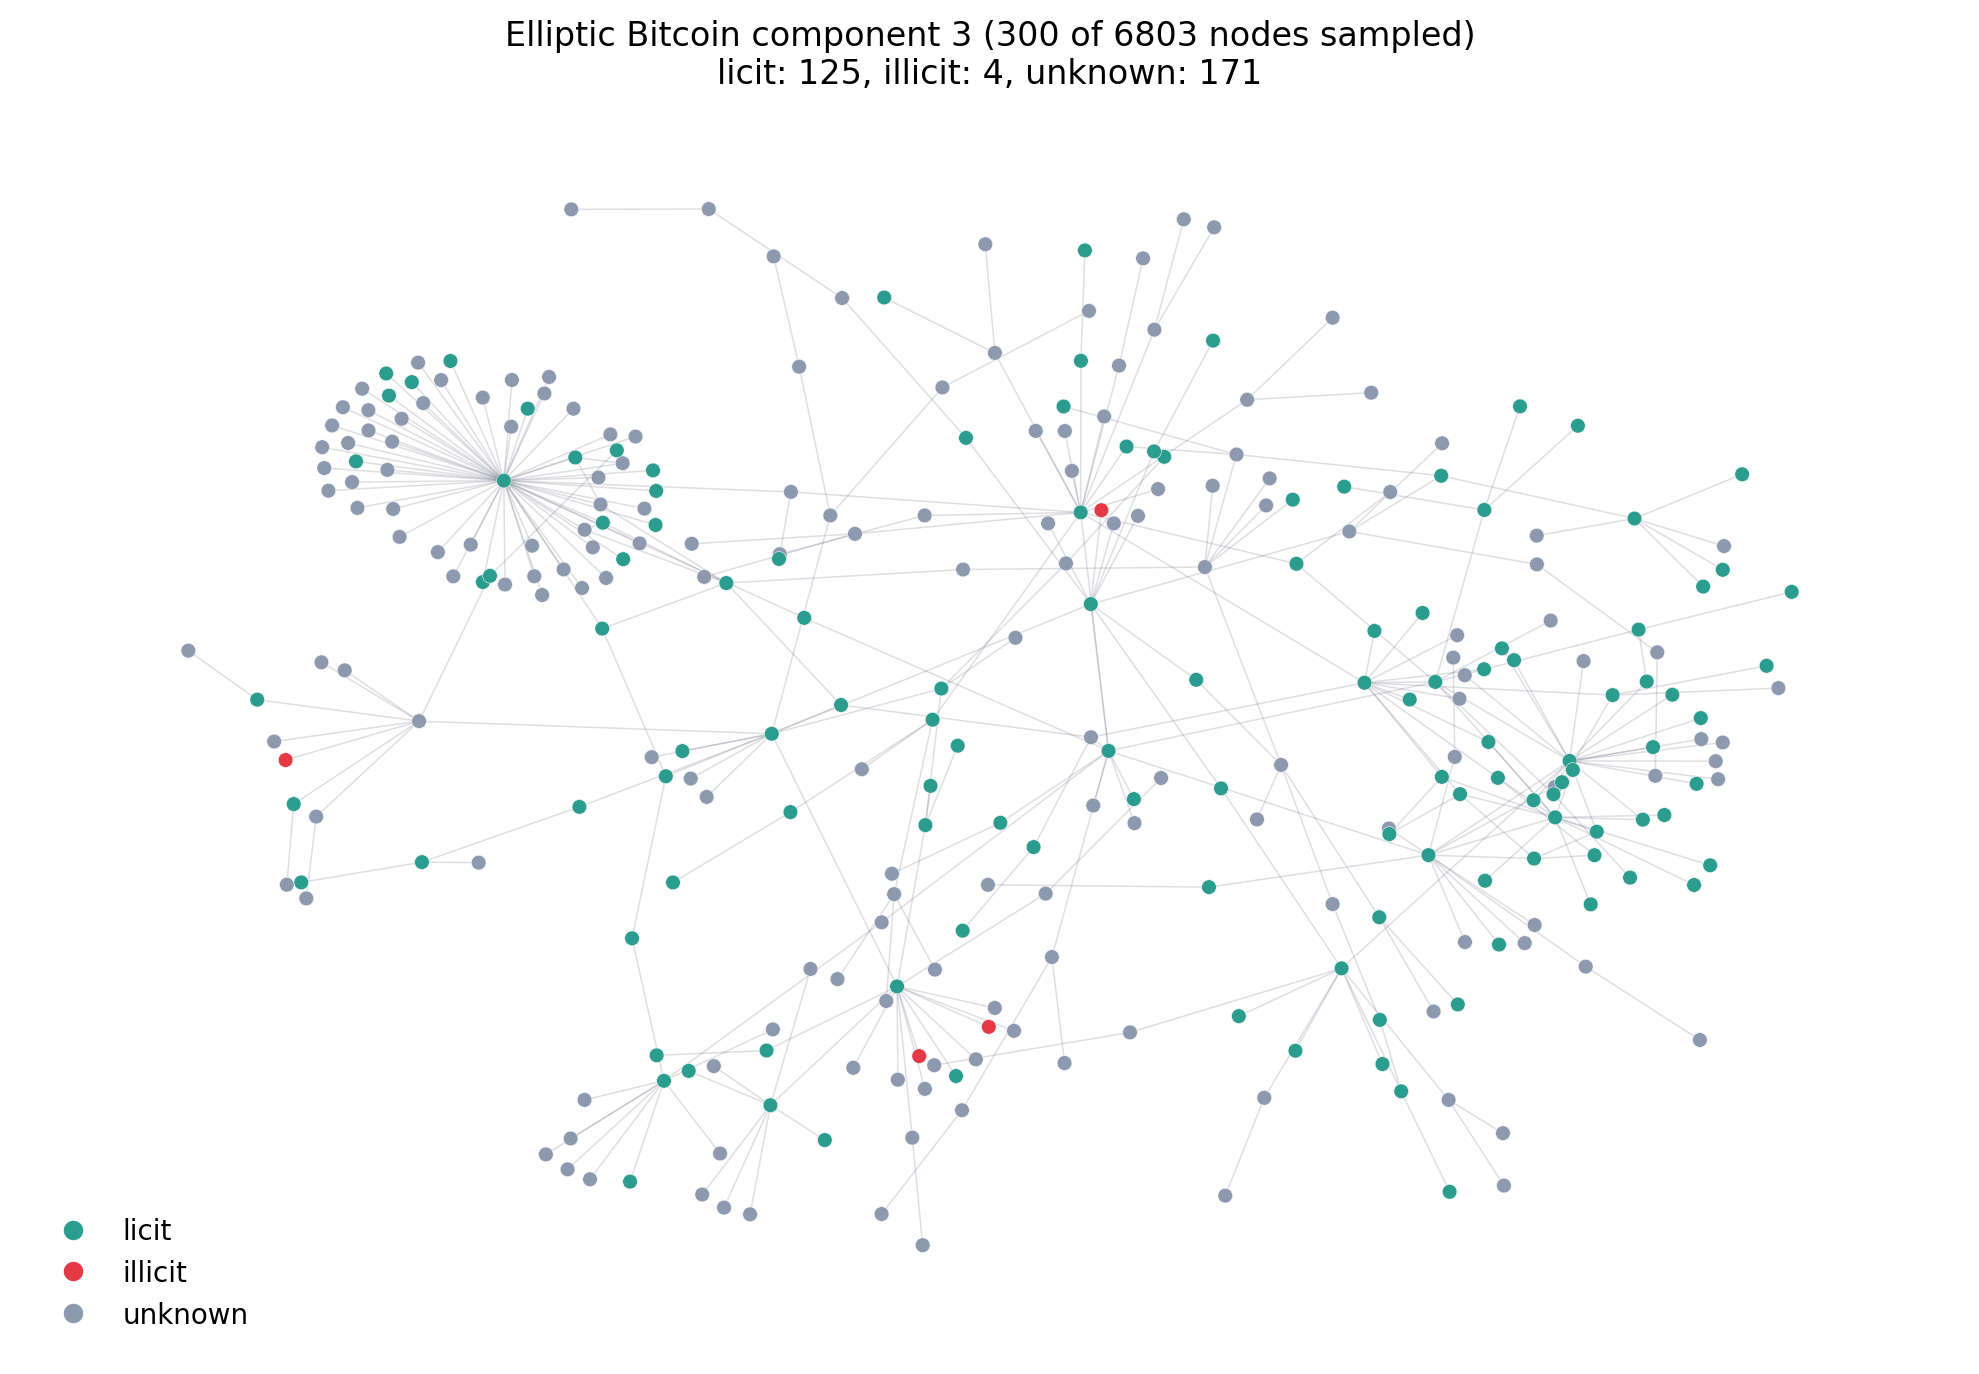
\includegraphics[width=\textwidth]{figures/elliptic_components/component_03.png}
        \label{fig:net_comp1}
    \end{subfigure}
    \hfill
    \begin{subfigure}[b]{0.48\textwidth}
        \centering
        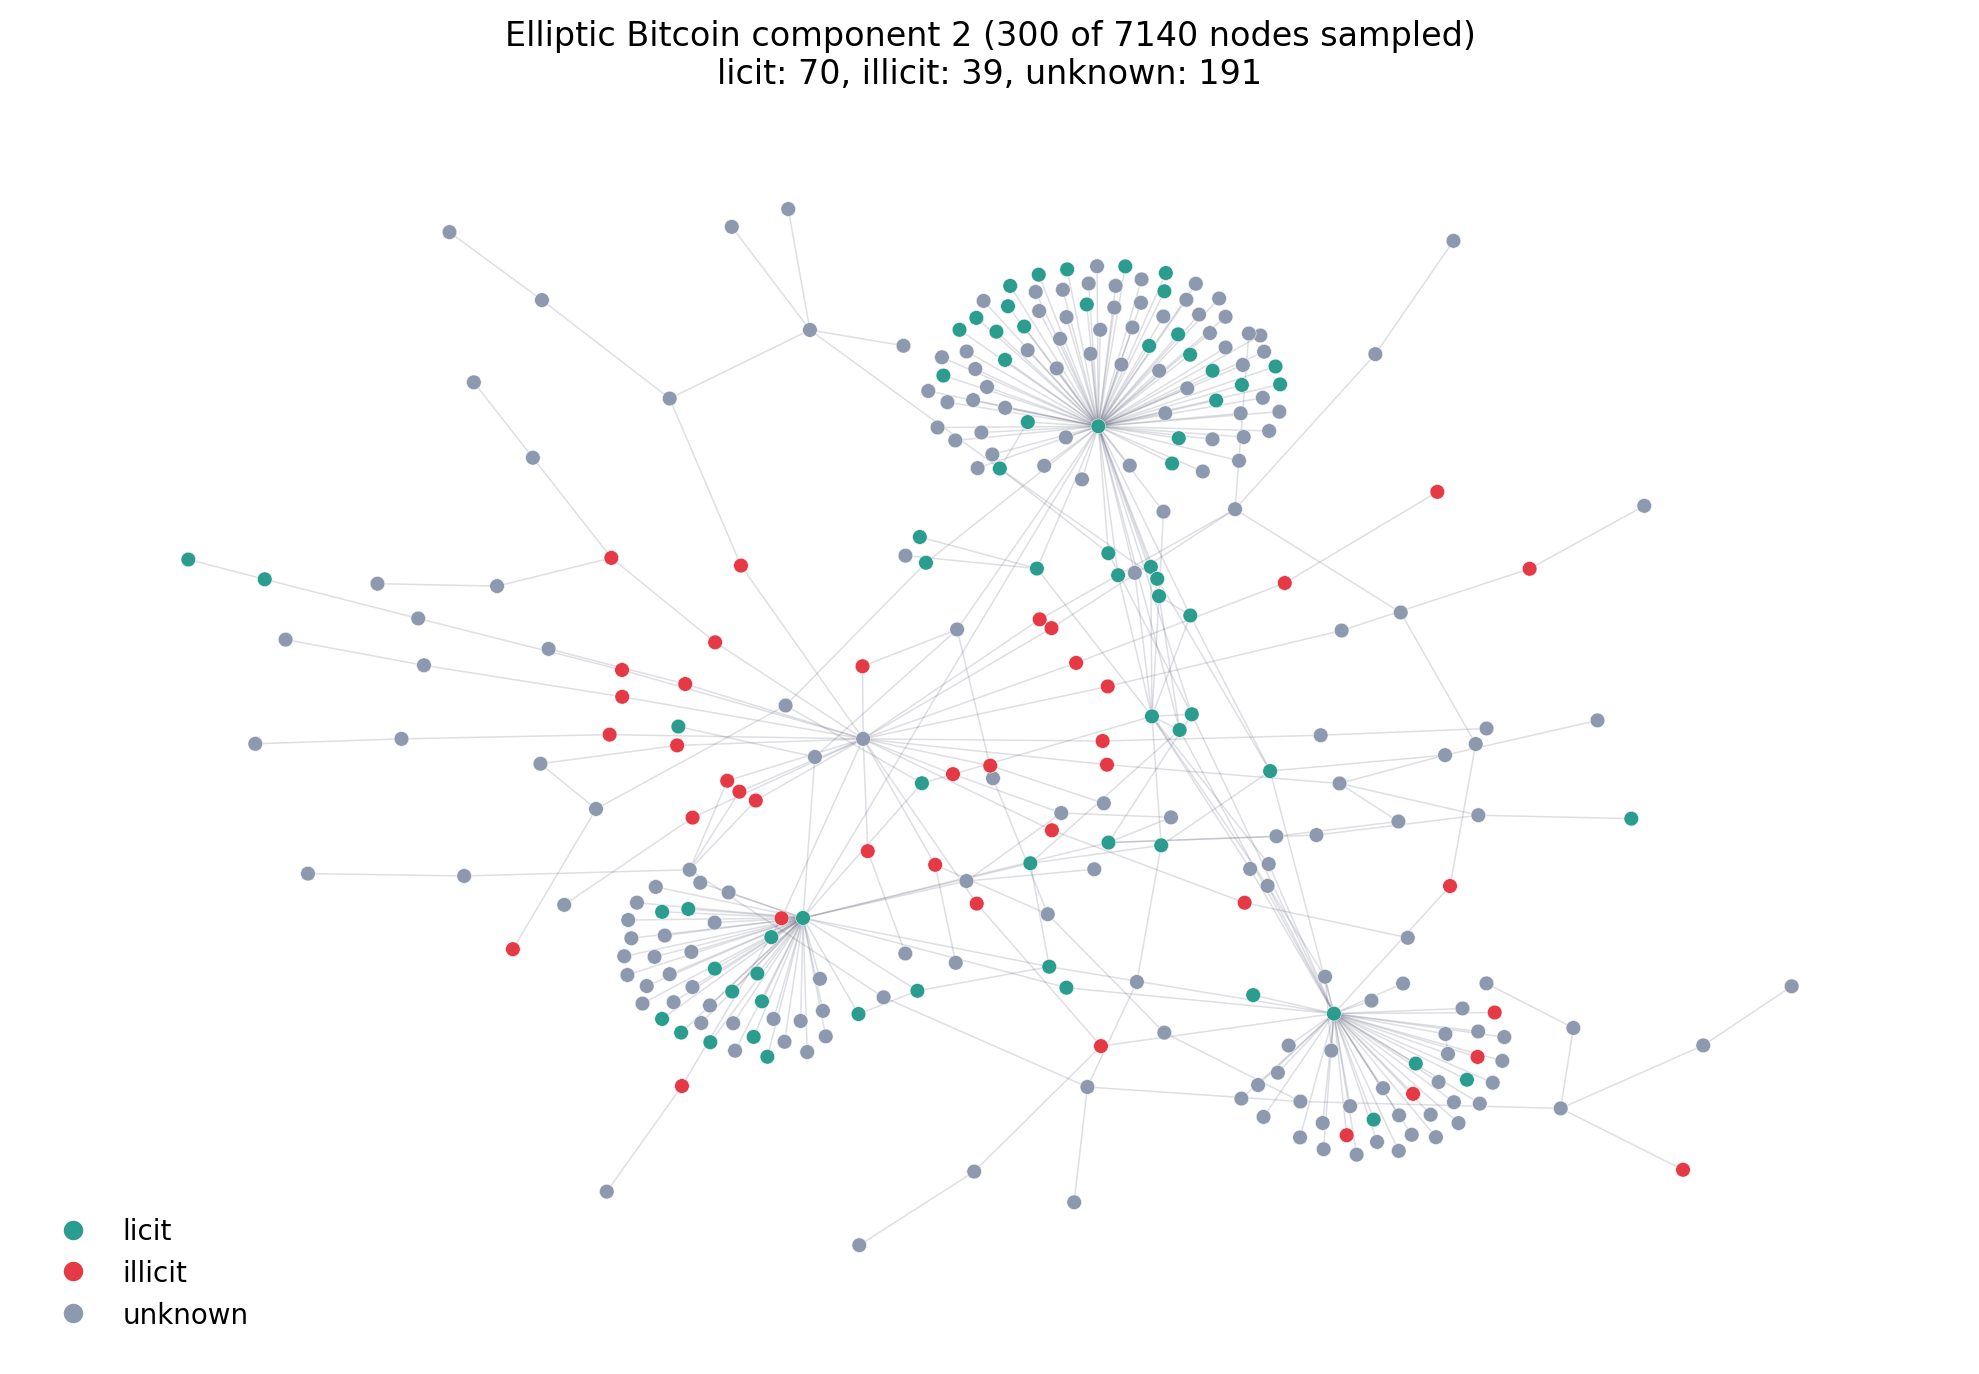
\includegraphics[width=\textwidth]{figures/elliptic_components/component_02.png}
        \label{fig:net_comp2}
    \end{subfigure}
    \caption{Visualization of network components and the labels.}
\end{figure}
\end{frame}

\begin{frame}{What do \Cref{fig:net_comp1,fig:net_comp2} suggest?}
\small
\begin{itemize}
    \item \Cref{fig:net_comp} displays part of one of the \textbf{49 connected components} in the graph.
    \item The displayed component suggests that the graph contains relatively few cycles.
    \item A large number of nodes have \textbf{unknown labels}, shown in gray.
\end{itemize}

\begin{frame}{Heatmap}
    \begin{figure}[b]{0.4\textwidth}
         \centering
         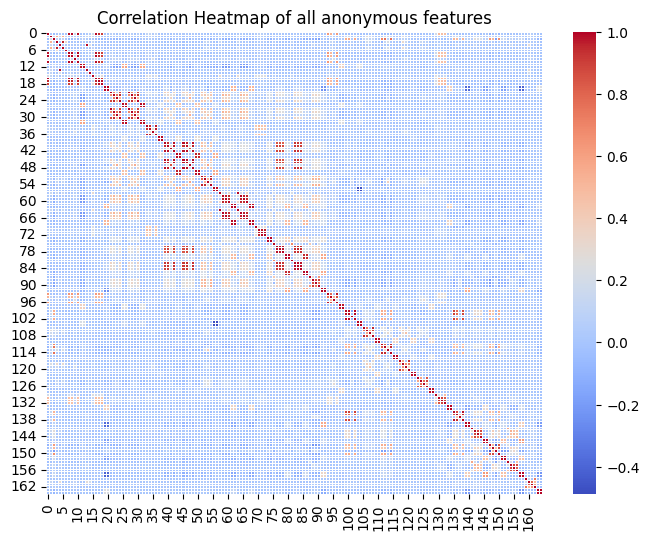
\includegraphics[width=\textwidth]{figures/feature_correlation.png}
         \caption{Correlation heatmap of features}
         \label{fig:heatmap}
     \caption{Visualization of feature correlations.}
     \end{figure}
\end{frame}

\begin{frame}{What do \Cref{fig:heatmap} suggest?}
    \begin{itemize}
        \item \Cref{fig:heatmap} indicates that most anonymous features are only weakly correlated.
    \item At the same time, a few blocks of non-negligible correlation are visible, suggesting dependence and possible redundancy among subsets of covariates.
    \end{itemize}
\end{frame}

% \centering
% \textbf{Takeaway:} both network structure and node-level covariates appear informative.
% \end{frame}

\begin{frame}{Neighborhood-level summaries}
\small
\begin{table}
\centering
\caption{Example node-level neighborhood features}
\begin{tabular}{rrrrrr}
\toprule
idx & node & node label & labeled neighbors & illicit neighbors & \% illicit neighbor \\
\midrule
0   & 3    & licit   & 62 & 1 & 0.0161 \\
1   & 9    & licit   & 23 & 0 & 0.0    \\
2   & 10   & licit   & 2  & 0 & 0.0    \\
263 & 907  & illicit & 1  & 0 & 0.0    \\
391 & 1361 & illicit & 1  & 0 & 0.0    \\
\bottomrule
\end{tabular}
\label{table:node}
\end{table}

\vspace{-0.25cm}
\begin{itemize}
    \item \Cref{table:node} illustrates the neighborhood features used in the analysis.
    \item We next aggregate these summaries by node label.
\end{itemize}
\end{frame}

\begin{frame}{Homophily evidence from \Cref{table:neighbor,table:transition}}
\small
\begin{columns}[T]
\begin{column}{0.62\textwidth}
\begin{table}
\centering
\caption{Neighborhood summary by node label}
\begin{tabular}{lrrrrr}
\toprule
node label & nodes & labeled neighbor & illicit neighbor & \% illicit neighbor & \% has illicit neighbor \\
\midrule
illicit & 4545  & 0.8123 & 0.4392 & 0.5097 & 0.3001 \\
licit   & 42019 & 1.6553 & 0.0404 & 0.0181 & 0.0244 \\
\bottomrule
\end{tabular}
\label{table:neighbor}
\end{table}
\end{column}
\begin{column}{0.34\textwidth}
\begin{table}
\centering
\caption{Transition counts between labeled source and target nodes}
\begin{tabular}{lrr}
\toprule
source/target & licit & illicit \\
\midrule
licit   & 33930 & 1228 \\
illicit & 468   & 998  \\
\bottomrule
\end{tabular}
\label{table:transition}
\end{table}
\end{column}
\end{columns}

\vspace{-0.1cm}
\begin{itemize}
    \item Illicit transactions have a much larger proportion of illicit neighbors.
    \item Same-class edges occur much more frequently than cross-class edges.
    \item This is consistent with a strong \alert{homophily effect} in the network.
\end{itemize}
\end{frame}

\begin{frame}{Refined model sketch}
\small
Assume $\sigma_i \in \{-1,1\}$ is the label of transaction $i$, where $-1$ denotes the illicit class and $1$ denotes the licit class.

\vspace{0.15cm}
We model the joint law of the labels given the features $X$ and graph $G$ by
\[
    P(\sigma_1,\sigma_2,\ldots,\sigma_n \mid X,G)
    \propto \prod_{(i,j)\in E} \psi_{X_i,X_j}(\sigma_i,\sigma_j).
\]

For binary labels, write the symmetric pairwise potential as
\[
    \psi_{X_i,X_j}(\sigma_i,\sigma_j)
    = \exp\!\left(\beta_{ij}\sigma_i\sigma_j + \alpha_{ij}(\sigma_i+\sigma_j) + c_{ij}\right).
\]

Assuming a common network parameter $\beta_{ij}=\beta$ for all $(i,j)\in E$, we obtain
\[
P(\sigma \mid X,G)
\propto
\exp\!\left(
\beta \sum_{(i,j)\in E} \sigma_i\sigma_j
+ 2\sum_{i=1}^n \sigma_i \sum_{j:(i,j)\in E} \alpha_{ij}
\right).
\]
\end{frame}

\begin{frame}{Covariate effect and final form}
\small
Model the node-level effect by
\[
    \sum_{j:(i,j)\in E} \alpha_{ij} = X_i^T\gamma,
\]
where $\gamma$ captures the effect of the anonymous features on the labels.

\vspace{0.2cm}
Substituting this into the previous expression gives
\[
    P(\sigma_1,\sigma_2,\ldots,\sigma_n \mid X,G)
    \propto
    \exp\!\left(
        \beta \sum_{(i,j)\in E} \sigma_i\sigma_j
        + 2\sum_{i=1}^n \sigma_i X_i^T\gamma
    \right).
\]

\begin{itemize}
    \item The first term encodes \alert{network dependence}.
    \item The second term encodes the contribution of \alert{node-level covariates}.
    \item The EDA in \Cref{fig:net_comp,fig:heatmap,table:neighbor,table:transition} motivates using both terms.
\end{itemize}
\end{frame}

\begin{frame}{Takeaways}
\begin{itemize}
    \item The Bitcoin transaction graph is large, sparse, and only partially labeled.
    \item \Cref{fig:net_comp,fig:heatmap} suggest that both graph structure and feature information are relevant.
    \item \Cref{table:neighbor,table:transition} provide strong empirical evidence of homophily.
    \item This motivates a model that combines:
    \begin{itemize}
        \item a covariate term through $\gamma$, and
        \item a network interaction term through $\beta$.
    \end{itemize}
    \item Next step: estimate the parameters and compare with feature-only baselines.
\end{itemize}
\end{frame}

\begin{frame}{References}
\footnotesize
\begin{thebibliography}{9}
\bibitem{daskalakis2020logistic}
Constantinos Daskalakis, Nishanth Dikkala, and Ioannis Panageas.
\newblock Logistic regression with peer-group effects via inference in higher-order Ising models.
\newblock \emph{International Conference on Artificial Intelligence and Statistics}, 2020.

\bibitem{mukherjee2024logistic}
Somabha Mukherjee, Ziang Niu, Sagnik Halder, Bhaswar B. Bhattacharya, and George Michailidis.
\newblock Logistic regression under network dependence.
\newblock \emph{Journal of Machine Learning Research}, 25(411):1--62, 2024.

\bibitem{weber2019antimoneylaunderingbitcoinexperimenting}
Mark Weber, Giacomo Domeniconi, Jie Chen, Daniel Karl I. Weidele, Claudio Bellei, Tom Robinson, and Charles E. Leiserson.
\newblock Anti-money laundering in bitcoin: Experimenting with graph convolutional networks for financial forensics.
\newblock 2019.
\end{thebibliography}
\end{frame}

\end{document}
